\documentclass[tikz, border=10pt]{standalone}
\usepackage{tikz}
    \usetikzlibrary{3d, angles, arrows, arrows.meta, babel, backgrounds, bending, calc, circuits.logic.US, decorations.markings, decorations.pathmorphing, decorations.pathreplacing, decorations.text, decorations, er, fit, graphs, intersections, matrix, mindmap, patterns, plotmarks, positioning, quotes, svg.path, shadows.blur, shapes.misc, tikzmark, trees, shapes, shadows, through, circuits.logic.US, circuits.logic.IEC, circuits.logic.CDH, circuits.ee.IEC}
\usepackage{tkz-euclide}

\usepackage{pgf}
	\usepgflibrary{decorations.text}
\usepackage{pgfplots}
	\pgfplotsset{compat=newest}

\usepackage{siunitx}						        % A comprehensive (SI) units package
	\sisetup{output-decimal-marker = {,}}	% Komma als Dezimaltrennzeichen für siunitx
	\sisetup{exponent-product = \cdot}		% Punkt statt x zwischen Zahl und Zehnerpotenz
	\sisetup{per-mode = fraction, fraction-function=\tfrac}			% Bruchstrich in Einheit
	\sisetup{inter-unit-product = \cdot}
	\sisetup{detect-weight=true, detect-family=true} 
	\sisetup{detect-all=true}             % für fettes SI - Quelle: https://tex.stackexchange.com/questions/610211/how-to-have-bold-unit-with-siunitx

\begin{document}

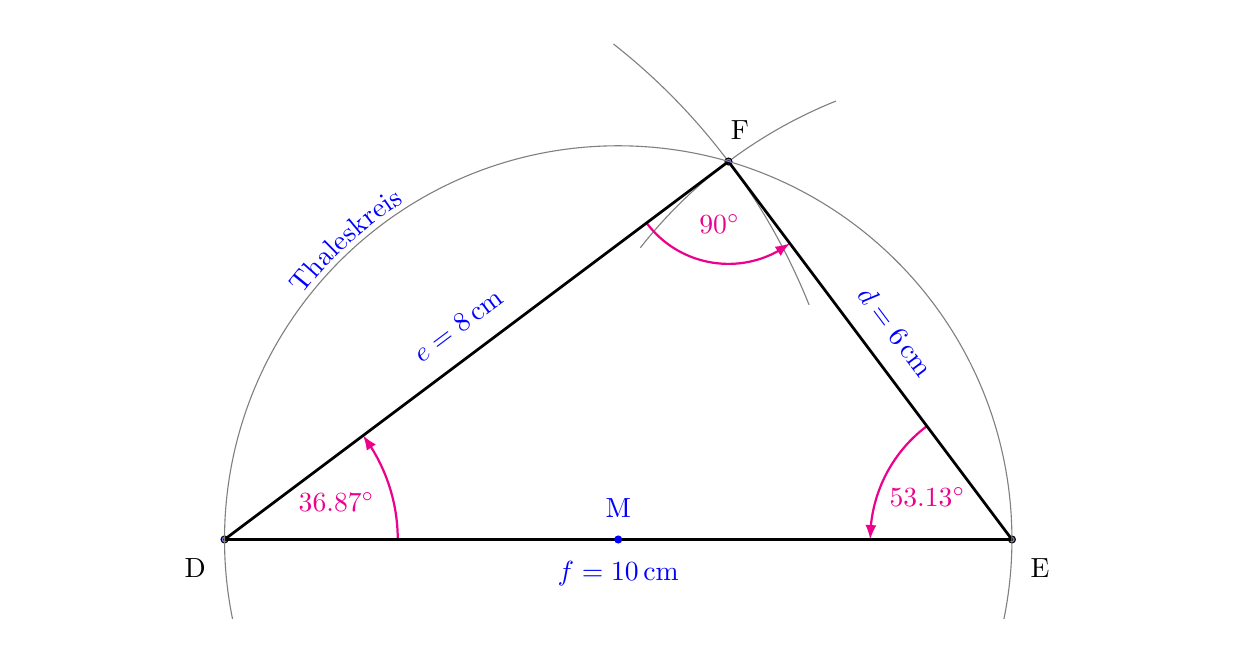
\begin{tikzpicture}%[show background grid]

%%% Definitionen der Styles
\tkzSetUpColors[background = white, text = black] 
\tkzSetUpPoint[size = 2.5pt, color = black, fill = blue!50] % war size=2.5pt
\tkzSetUpLine[line width = 1pt, color = black, line cap = round] 
\tkzSetUpCompass[color = gray, line width =.4 pt, delta = 15]
\tkzSetUpArc[color = gray, line width = .4pt] 
\tkzSetUpStyle[orange]{new}

%%% Definition der BoundingBox x=11 y=7
\useasboundingbox (-2,-1) rectangle (13,6.5);

%%% Beschnitt auf die BoundingBox
\tkzClipBB

%%% Definition von Punkten
\tkzDefPoint(0.5,0){A}	
\tkzDefPoint(10.5,0){B}

%%% Schneiden zweier Kreise
\tkzInterCC[R](A,8)(B,6) \tkzGetFirstPoint{C}

%%% Zeichnen von Kreisen
\tkzCompass(A,C)
\tkzCompass(B,C)

%%%% Winkel mit Pfeil markieren und anschließend beschriften 
%\tkzMarkRightAngle[-latex, color=magenta, size=.75, draw, thick, german](S1,A,C)
\tkzFindAngle(B,A,C)   \tkzGetAngle{winkelalpha}
\tkzMarkAngle[-latex, color = magenta, size = 2.2, draw,  thick](B,A,C)
	\tkzLabelAngle[color = magenta, pos=1.5](B,A,C){$ \pgfmathprintnumber{\winkelalpha}\si{\degree}$}

\tkzFindAngle(C,B,A)   \tkzGetAngle{winkelbeta}
\tkzMarkAngle[-latex, color = magenta, size = 1.8, draw,  thick](C,B,A)
	\tkzLabelAngle[color = magenta, pos=1.2](C,B,A){$ \pgfmathprintnumber{\winkelbeta}\si{\degree}$}

\tkzFindAngle(A,C,B)   \tkzGetAngle{winkelgamma}	
\tkzMarkAngle[-latex, color = magenta, size = 1.3, draw,  thick](A,C,B)
	\tkzLabelAngle[color = magenta, pos=0.8](A,C,B){$ \pgfmathprintnumber{\winkelgamma}\si{\degree}$}

%%% Zeichnen von Punkten	
\tkzDrawPoint(A)	\tkzLabelPoint[below left = 1ex, color = black](A){D} 
\tkzDrawPoint(B)	\tkzLabelPoint[below right = 1ex, color = black](B){E} 
\tkzDrawPoint(C)	\tkzLabelPoint[above = 1ex, color = black](C){\;\;\;F} 

%%% Berechnen von Streckenlängen
\tkzCalcLength(A,B)	\tkzGetLength{rAB}	
\tkzCalcLength(B,C)	\tkzGetLength{rBC}	
\tkzCalcLength(A,C)	\tkzGetLength{rAC}	

%%% Zeichnen von Strecken
\tkzDrawSegment[line cap = round](A,B)	
\tkzLabelSegment[below = 1ex, color = blue, sloped](A,B){$f=\SI{\rAB}{\centi \meter}$}

\tkzDrawSegment[line cap=round](B,C)	
\tkzLabelSegment[above = 1ex, color = blue, sloped](B,C){$d=\SI{\rBC}{\centi \meter}$}

\tkzDrawSegment[line cap=round](A,C)	
\tkzLabelSegment[above = 1ex, color = blue, sloped](A,C){$e=\SI{\rAC}{\centi \meter}$}

%%% Zeichnen des Thaleskreises
\tkzDefMidPoint(A,B) 	\tkzGetPoint{M}		\tkzDrawPoints[color=blue](M)	\tkzLabelPoint[above=1ex, color=blue](M){M}
\tkzDrawCircle[color = gray, thin,
    postaction={decoration = {
		reverse path,,
		raise=0.5ex ,
		text along path ,
		text color=blue ,
		text={Thaleskreis} ,
		text align={left indent=190mm}} , decorate
    }
](M,A)
\end{tikzpicture}
\end{document}
